\documentclass[10pt,final]{beamer}
\mode<presentation>
\usetheme{debian}

%Translators:
%change debiantutorial to debiantutorial.$lang to use translated file, and
%append to this string all commands to load localisation packages, e.g.:
%\\usepackage{debiantutorial.fr} \\usepackage[french]{babel} \\frenchsetup{...}
\usepackage{debiantutorial}

\hypersetup{bookmarks}
\title{Debian Packaging Tutorial}
\author[]{Lucas Nussbaum\\{\small\texttt{packaging-tutorial@packages.debian.org}}}

%Translators:
%leave \\version unchanged: this will a variable containing the actual version
%To translate the date, use \\today or a string containing \\year, \\month, \\day
%(numeric values).
\date{\footnotesize version 0.9 -- 2013-06-20} % DATE - use debian/rules update-version-date

\begin{document}


\frame{\titlepage}

\begin{frame}{About this tutorial}
  \begin{itemize}
  \item Goal: \textbf{tell you what you really need to know about Debian packaging}
    \begin{itemize}
      \hbr
    \item Modify existing packages
      \hbr
    \item Create your own packages
	    \hbr
    \item Interact with the Debian community
      \hbr
    \item Become a Debian power-user
    \end{itemize}
    \br
  \item Covers the most important points, but is not complete
    \begin{itemize}
    \item You will need to read more documentation
    \end{itemize}
    \br
  \item Most of the content also applies to Debian derivative distributions
    \begin{itemize}
      \hbr
    \item That includes Ubuntu
    \end{itemize}
  \end{itemize}
\end{frame}

\begin{frame}{Outline}
  \tableofcontents[hideallsubsections]
\end{frame}

\section{Introduction}

\subsection{Debian}

\begin{frame}{Debian}
	\begin{itemize}
		\item \textbf{GNU/Linux distribution}
			\br
		\item 1st major distro developed ``openly in the spirit of GNU''
			\br
		\item \textbf{Non-commercial}, built collaboratively by over 1,000 volunteers
			\br
		\item 3 main features:
			\begin{itemize}
				\item \textbf{Quality} -- culture of technical excellence\\
					{\small\sl We release when it's ready}
					\hbr
				\item \textbf{Freedom} -- devs and users bound by the \textsl{Social Contract}\\
					Promoting the culture of Free Software since 1993
					\hbr
				\item \textbf{Independence} -- no (single) company babysitting Debian\\
					And open decision-making process (\textsl{do-ocracy} + \textsl{democracy})
			\end{itemize}
                        \br
                \item \textbf{Amateur} in the best sense: done for the love of it
	\end{itemize}
\end{frame}

\subsection{Debian packages}
\begin{frame}{Debian packages}
\begin{itemize}
\item \textbf{.deb} files (binary packages)
	\br
\item A very powerful and convenient way to distribute software to users
	\br
\item One of the two most common package formats (with RPM)
	\br
\item Universal:
	\begin{itemize}
		\item 30,000 binary packages in Debian\\
			$\rightarrow$ most of the available free software is packaged in Debian!
			\hbr
		\item For 12 ports (architectures), including 2 non-Linux (Hurd; KFreeBSD)
			\hbr
		\item Also used by 120 Debian derivative distributions
	\end{itemize}
\end{itemize}
\end{frame}


\subsection{The Deb package format}

\begin{frame}[fragile=singleslide]{The Deb package format}
  \begin{itemize}
  \item \texttt{.deb} file: an \texttt{ar} archive
    \begin{lstlisting}[basicstyle=\ttfamily\footnotesize]
$ ar tv wget_1.12-2.1_i386.deb
rw-r--r-- 0/0      4 Sep  5 15:43 2010 debian-binary
rw-r--r-- 0/0   2403 Sep  5 15:43 2010 control.tar.gz
rw-r--r-- 0/0 751613 Sep  5 15:43 2010 data.tar.gz
    \end{lstlisting} % $
    \begin{itemize}
    \item \texttt{debian-binary}: version of the deb file format, \texttt{"2.0\textbackslash{}n"}
    \item \texttt{control.tar.gz}: metadata about the package\\
      {\small \texttt{\textbf{control}, md5sums, (pre|post)(rm|inst), triggers, shlibs}, \ldots}
    \item \texttt{data.tar.gz}: data files of the package
    \end{itemize}
    \br
  \item You could create your \texttt{.deb} files manually\\
    {\footnotesize \url{http://tldp.org/HOWTO/html\_single/Debian-Binary-Package-Building-HOWTO/}}
    \br
  \item But most people don't do it that way
  \end{itemize}
  \br
  \centerline{\textbf{This tutorial: create Debian packages, the Debian way}}
\end{frame}

\subsection{Tools you will need}
\begin{frame}{Tools you will need}
  \begin{itemize}
  \item A Debian (or Ubuntu) system (with root access)
    \br
  \item Some packages:
    \begin{itemize}
    \item \textbf{build-essential}: has dependencies on the packages that will
      be assumed to be available on the developer's machine (no need to specify
      them in the \texttt{Build-Depends:} control field of your package)
      \begin{itemize}
      \item includes a dependency on \textbf{dpkg-dev}, which contains basic
        Debian-specific tools to create packages
      \end{itemize}
      \hbr
    \item \textbf{devscripts}: contains many useful scripts for Debian
      maintainers
    \end{itemize}
  \end{itemize}

  \br
  Many other tools will also be mentioned later, such as \textbf{debhelper},
  \textbf{cdbs}, \textbf{quilt}, \textbf{pbuilder}, \textbf{sbuild},
  \textbf{lintian}, \textbf{svn-buildpackage}, \textbf{git-buildpackage},
  \ldots\\
  Install them when you need them.
\end{frame}

\subsection{General packaging workflow}
\begin{frame}{General packaging workflow}
  \begin{center}
    \begin{tikzpicture}[
      node1/.style={shape=rectangle,draw=rouge,fill=debianbackgroundblue,thick},
      arr/.style={very thick}, command/.style={text=rouge,font=\ttfamily}, ]
      
      \node[node1] (www) at (0, 0) {Web};
      \node[node1] (us) at (2.5, 0) {upstream source};
      \node[node1] (da) at (-2.5, 0) {Debian mirror};
      \node[node1] (sp) at (0, -2) {source package};
      \draw[arr,<-,dashed,thick] (sp) -- (2.5,-2) node[right=0cm,text width=2.98cm,text centered,font=\small\sl] {where most of the manual work is done};
      \node[node1] (bin) at (0, -4) {one or several binary packages};
      \draw[arr,<-,dashed,thick] (bin) -- (3.5,-4) node[right,text centered,font=\small\ttfamily\sl] {.deb\normalfont};
      \draw[arr,->] (us) -- (sp) node[pos=0.5,right,command] {dh\_make};
      \draw[arr,->] (da) -- (sp) node[pos=0.5,left,command] {apt-get source};
      \draw[arr,->] (www) -- (sp) node[pos=0.5,left,command] {dget};
      \draw[arr,->] (sp) -- (bin) node[pos=0.5,right,text width=6cm] {\textttc{debuild} (build and test with \textttc{lintian}) or \textttc{dpkg-buildpackage}};
      \draw[arr,->] (bin) -- (1,-6) node[pos=0.5,right] {install (\textttc{debi})};
      %	\draw[arr,->] (bin) -- (-1,-6) node[pos=0.5,left] {upload (\textttc{dput})};
      \draw[transparent] (bin) -- (-1,-6) node[pos=0.5,left,opaque] {upload (\textttc{dput})};
      \draw[arr,->,rounded corners] (bin) -- (-1,-6) -- (-4.5,-6) -- (-4.5,0) -- (da);
      \useasboundingbox (-4,-6) rectangle (6,0); % hack hack hack
    \end{tikzpicture}
  \end{center}
\end{frame}

\subsection{Rebuilding dash}
\begin{frame}{Example: rebuilding dash}
\begin{enumerate}
\item Install packages needed to build dash, and devscripts\\
  {\texttt{sudo apt-get build-dep dash}\\ (requires \texttt{deb-src} lines in \texttt{/etc/apt/sources.list})}\\
  {\texttt{sudo apt-get install -{}-no-install-recommends devscripts fakeroot}}
  \hbr
\item Create a working directory, and get in it:\\
 \texttt{mkdir /tmp/debian-tutorial ; cd /tmp/debian-tutorial}
  \hbr
\item Grab the \texttt{dash} source package\\
  \texttt{apt-get source dash}\\ 
  {\small (This needs you to have \texttt{deb-src} lines in your \texttt{/etc/apt/sources.list})}
  \hbr
\item Build the package\\
  {\texttt{cd dash-*\\ debuild -us -uc}} ~~~(\texttt{-us -uc} disables signing the package with GPG)

  \hbr
\item Check that it worked
	\begin{itemize}
		\item  There are some new \texttt{.deb} files in the parent directory
	\end{itemize}
    \hbr
\item Look at the \texttt{debian/} directory
	\begin{itemize}
		\item That's where the packaging work is done
	\end{itemize}
\end{enumerate}
\end{frame}

\section{Creating source packages}
\subsection{Source packages basics}
\begin{frame}{Source package}
  \begin{itemize}
  \item One source package can generate several binary packages\\
    {\small e.g. the \texttt{\bfseries libtar} source generates the
      \texttt{\bfseries libtar0} and \texttt{\bfseries libtar-dev} binary
      packages} \hbr
  \item Two kinds of packages: (if unsure, use non-native)
    \begin{itemize}
      \small
    \item Native packages: normally for Debian specific software (\textsl{dpkg}, \textsl{apt})
    \item Non-native packages: software developed outside Debian
    \end{itemize}
    \hbr
  \item Main file: \texttt{.dsc} (meta-data)
    \hbr
  \item Other files depending on the version of the source format
    \begin{itemize}
    \item 1.0 or 3.0 (native): \texttt{package\_version.tar.gz}
      \hbr
    \item 1.0 (non-native):
      \begin{itemize}
      \item \texttt{pkg\_ver.orig.tar.gz}: upstream source
      \item \texttt{pkg\_debver.diff.gz}: patch to add Debian-specific changes
      \end{itemize}
      \hbr
    \item 3.0 (quilt):
      \begin{itemize}
      \item \texttt{pkg\_ver.orig.tar.gz}: upstream source
      \item \texttt{pkg\_debver.debian.tar.gz}: tarball with the Debian changes
      \end{itemize}
    \end{itemize}
  \end{itemize}
  \hbr
  (See \texttt{dpkg-source(1)} for exact details)
\end{frame}

\begin{frame}[fragile=singleslide]{Source package example (wget\_1.12-2.1.dsc)}
  \begin{lstlisting}[basicstyle=\ttfamily\small]
Format: 3.0 (quilt)
Source: wget
Binary: wget
Architecture: any
Version: 1.12-2.1
Maintainer: Noel Kothe <noel@debian.org>
Homepage: http://www.gnu.org/software/wget/
Standards-Version: 3.8.4
Build-Depends: debhelper (>> 5.0.0), gettext, texinfo,
 libssl-dev (>= 0.9.8), dpatch, info2man
Checksums-Sha1: 
 50d4ed2441e67[..]1ee0e94248 2464747 wget_1.12.orig.tar.gz
 d4c1c8bbe431d[..]dd7cef3611 48308 wget_1.12-2.1.debian.tar.gz
Checksums-Sha256: 
 7578ed0974e12[..]dcba65b572 2464747 wget_1.12.orig.tar.gz
 1e9b0c4c00eae[..]89c402ad78 48308 wget_1.12-2.1.debian.tar.gz
Files: 
 141461b9c04e4[..]9d1f2abf83 2464747 wget_1.12.orig.tar.gz
 e93123c934e3c[..]2f380278c2 48308 wget_1.12-2.1.debian.tar.gz
\end{lstlisting}
\end{frame}

\subsection{Retrieving source packages}
\begin{frame}{Retrieving an existing source package}
  \begin{itemize}
  \item From the Debian archive:
    \begin{itemize}
    \item \texttt{apt-get source \textsl{package}}
    \item \texttt{apt-get source \textsl{package=version}}
    \item \texttt{apt-get source \textsl{package/release}}
    \end{itemize}
    (You need \texttt{deb-src} lines in \texttt{sources.list})
    \br
  \item From the Internet:
    \begin{itemize}
    \item \texttt{dget \textsl{url-to.dsc}}
    \item \texttt{dget http://snapshot.debian.org/archive/debian-archive/\\20090802T004153Z/debian/dists/bo/main/source/web/\\
        wget\_1.4.4-6.dsc}\\ 
      (\href{http://snapshot.debian.org/}{\ttfamily snapshot.d.o} provides all packages from Debian since 2005)
    \end{itemize}
    \br
  \item From the (declared) version control system:
    \begin{itemize}
    \item \texttt{debcheckout \textsl{package}}
    \end{itemize}
    \br
  \item Once downloaded, extract with \texttt{dpkg-source -x \textsl{file.dsc}}
  \end{itemize}
\end{frame}

\subsection{Creating a basic source package}
\begin{frame}{Creating a basic source package}
  \begin{itemize}
  \item Download the upstream source\\
    (\textsl{upstream source} = the one from the software's original developers)
    \hbr
  \item Rename to \texttt{<\textsl{source\_package}>\_<\textsl{upstream\_version}>.orig.tar.gz}\\
    (example: \texttt{simgrid\_3.6.orig.tar.gz})
    \hbr
  \item Untar it
    \hbr
  \item Rename the directory to \texttt{<\textsl{source\_package}>-<\textsl{upstream\_version}>}\\
	  (example: \texttt{simgrid-3.6})
    \hbr
  \item \texttt{cd \texttt{<\textsl{source\_package}>-<\textsl{upstream\_version}>} \&\& dh\_make}\\
	  (from the \textbf{dh-make} package)
    \hbr
  \item There are some alternatives to \texttt{dh\_make} for specific sets of
    packages: \textbf{dh-make-perl}, \textbf{dh-make-php}, \ldots \hbr
  \item \texttt{debian/} directory created, with a lot of files in it
  \end{itemize}
\end{frame}

\subsection{Files in debian/}
\begin{frame}{Files in debian/}
  All the packaging work should be made by modifying files in \texttt{debian/}
  \hbr
  \begin{itemize}
  \item Main files:
    \begin{itemize}
    \item \textbf{control} -- meta-data about the package (dependencies, etc.)
    \item \textbf{rules} -- specifies how to build the package
    \item \textbf{copyright} -- copyright information for the package
    \item \textbf{changelog} -- history of the Debian package
    \end{itemize}
    \hbr
  \item Other files:
    \begin{itemize}
    \item compat
    \item watch
    \item dh\_install* targets\\
      {\small *.dirs, *.docs, *.manpages, \ldots}
    \item maintainer scripts\\
      {\small *.postinst, *.prerm, \ldots}
    \item source/format
    \item patches/ -- if you need to modify the upstream sources
    \end{itemize}
    \hbr
  \item Several files use a format based on RFC 822 (mail headers)
  \end{itemize}
\end{frame}

\begin{frame}[fragile=singleslide]{debian/changelog}
  \begin{itemize}
  \item Lists the Debian packaging changes
  \item Gives the current version of the package
  \begin{center}
    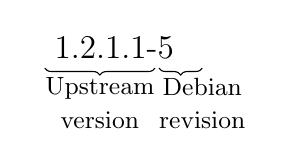
\begin{tikzpicture}
	    \draw (0,0) node[above right] {\large 1.2.1.1-5};
	    \draw [decorate,decoration={brace}] (2,0) -- (1.45,0) node[at start,below,text width=1.6cm,text centered] {\small  Debian revision};
	    \draw [decorate,decoration={brace}] (1.4,0) -- (0,0) node[midway,below,text width=1.6cm,text centered] { \small Upstream version};
\end{tikzpicture}
\end{center}


	  %%
  \item Edited manually or with \textttc{dch}
  \begin{itemize}
	  \item Create a changelog entry for a new release: \textttc{dch -i}
  \end{itemize}
  \item Special format to automatically close Debian or Ubuntu bugs\\
    Debian: \texttt{Closes:~\#595268}; Ubuntu: \texttt{LP:~\#616929}
  \item Installed as \texttt{/usr/share/doc/\textit{package}/changelog.Debian.gz}
  \end{itemize}
  \seprule
  \begin{lstlisting}[basicstyle=\ttfamily\footnotesize]
mpich2 (1.2.1.1-5) unstable; urgency=low

  * Use /usr/bin/python instead of /usr/bin/python2.5. Allow
    to drop dependency on python2.5.  Closes: #595268
  * Make /usr/bin/mpdroot setuid. This is the default after
    the installation of mpich2 from source, too. LP: #616929
    + Add corresponding lintian override.

 -- Lucas Nussbaum <lucas@debian.org>  Wed, 15 Sep 2010 18:13:44 +0200
\end{lstlisting}
\end{frame}

\begin{frame}[fragile=singleslide]{debian/control}
  \hbr
  \begin{itemize}
  \item Package metadata
    \begin{itemize}
    \item For the source package itself
    \item For each binary package built from this source
    \end{itemize}
    \hbr
  \item Package name, section, priority, maintainer, uploaders,
    build-dependencies, dependencies, description, homepage, \ldots \hbr
  \item Documentation: Debian Policy chapter 5\\
    \url{http://www.debian.org/doc/debian-policy/ch-controlfields}
  \end{itemize}
  \seprule
\begin{lstlisting}[basicstyle=\ttfamily\footnotesize]
Source: wget
Section: web
Priority: important
Maintainer: Noel Kothe <noel@debian.org>
Build-Depends: debhelper (>> 5.0.0), gettext, texinfo,
 libssl-dev (>= 0.9.8), dpatch, info2man
Standards-Version: 3.8.4
Homepage: http://www.gnu.org/software/wget/

Package: wget
Architecture: any
Depends: ${shlibs:Depends}, ${misc:Depends}
Description: retrieves files from the web
 Wget is a network utility to retrieve files from the Web
\end{lstlisting}
\end{frame}

\begin{frame}{Architecture: all or any}
  Two kinds of binary packages:
  \hbr
  \begin{itemize}
  \item Packages with different contents on each Debian architecture
    \begin{itemize}
    \item Example: C program
    \item \texttt{Architecture:\ any} in \texttt{debian/control}
      \begin{itemize}
      \item Or, if it only works on a subset of architectures:\\
        \texttt{Architecture:\ amd64 i386 ia64 hurd-i386}
      \end{itemize}
    \item buildd.debian.org: builds all the other architectures for you on upload
    \item Named \texttt{\textsl{package}\_\textsl{version}\_\textsl{architecture}.deb}
    \end{itemize}
    \br
  \item Packages with the same content on all architectures
    \begin{itemize}
    \item Example: Perl library
    \item \texttt{Architecture:\ all} in \texttt{debian/control}
    \item Named \texttt{\textsl{package}\_\textsl{version}\_\textbf{all}.deb}
    \end{itemize}
  \end{itemize}
  \br
  A source package can generate a mix of \texttt{Architecture:\ any} and \texttt{Architecture:\ all} binary packages
\end{frame}

\begin{frame}[fragile=singleslide]{debian/rules}
  \hbr
  \begin{itemize}
  \item Makefile
    \br
  \item Interface used to build Debian packages
    \br
  \item Documented in Debian Policy, chapter 4.8\\
    {\small \url{http://www.debian.org/doc/debian-policy/ch-source\#s-debianrules}}
    \br
  \item Required targets:
    \begin{itemize}
    \item \texttt{build, build-arch, build-indep}: should perform all the configuration and compilation
      \hbr
    \item \texttt{binary, binary-arch, binary-indep}: build the binary packages
      \begin{itemize}
      \item \texttt{dpkg-buildpackage} will call \texttt{binary} to build all
        the packages, or \texttt{binary-arch} to build only the
        \texttt{Architecture:~any} packages
      \end{itemize}
      \hbr
    \item \texttt{clean}: clean up the source directory
    \end{itemize}
  \end{itemize}
\end{frame}

\subsection{Packaging helpers}
\begin{frame}{Packaging helpers -- debhelper}
  \begin{itemize}
  \item You could write shell code in \texttt{debian/rules} directly
    \begin{itemize}
    \item See the \texttt{adduser} package for example
    \end{itemize}
    \hbr
  \item Better practice (used by most packages): use a \textsl{Packaging helper}
    \hbr
  \item Most popular one: \textbf{debhelper} (used by 98\% of packages)
    \hbr
  \item Goals:
    \begin{itemize}
    \item Factor the common tasks in standard tools used by all packages
    \item Fix some packaging bugs once for all packages
    \end{itemize}
    {\footnotesize dh\_installdirs, dh\_installchangelogs, dh\_installdocs,
      dh\_installexamples, dh\_install, dh\_installdebconf, dh\_installinit,
      dh\_link, dh\_strip, dh\_compress, dh\_fixperms, dh\_perl,
      dh\_makeshlibs, dh\_installdeb, dh\_shlibdeps, dh\_gencontrol,
      dh\_md5sums, dh\_builddeb, \ldots}
    \begin{itemize}
    \item Called from \texttt{debian/rules}
    \item Configurable using command parameters or files in \texttt{debian/}
    \end{itemize}
    {\footnotesize \ttfamily \textsl{package}.docs, \textsl{package}.examples,
      \textsl{package}.install, \textsl{package}.manpages, \ldots} \hbr
  \item Third-party helpers for sets of packages: \textbf{python-support},
    \textbf{dh\_ocaml}, \ldots \hbr
  \item Gotcha: \texttt{debian/compat}: Debhelper compatibility version (use "7")
  \end{itemize}
\end{frame}

\begin{frame}[fragile=singleslide]{debian/rules using debhelper (1/2)}
  \begin{lstlisting}[basicstyle=\ttfamily\footnotesize,escapeinside=\{\}]
#!/usr/bin/make -f

# Uncomment this to turn on verbose mode.
#export DH_VERBOSE=1

build: 
        $(MAKE)
        #docbook-to-man debian/packagename.sgml > packagename.1

clean: 
        dh_testdir
        dh_testroot
        rm -f build-stamp configure-stamp
        $(MAKE) clean
        dh_clean 

install: build
        dh_testdir
        dh_testroot
        dh_clean -k 
        dh_installdirs
        # Add here commands to install the package into debian/packagename.
        $(MAKE) DESTDIR=$(CURDIR)/debian/packagename install
\end{lstlisting}
\end{frame}

\begin{frame}[fragile=singleslide]{debian/rules using debhelper (2/2)}
  \begin{lstlisting}[basicstyle=\ttfamily\footnotesize,escapeinside=\{\}]

# Build architecture-independent files here.
binary-indep: build install

# Build architecture-dependent files here.
binary-arch: build install
        dh_testdir
        dh_testroot
        dh_installchangelogs 
        dh_installdocs
        dh_installexamples
        dh_install
        dh_installman
        dh_link
        dh_strip
        dh_compress
        dh_fixperms
        dh_installdeb
        dh_shlibdeps
        dh_gencontrol
        dh_md5sums
        dh_builddeb

binary: binary-indep binary-arch
.PHONY: build clean binary-indep binary-arch binary install configure
\end{lstlisting}
\end{frame}

\begin{frame}[fragile=singleslide]{CDBS}
  \hbr
  \begin{itemize}
  \item With debhelper, still a lot of redundancy between packages
    \hbr
  \item Second-level helpers that factor common functionality
    \begin{itemize}
    \item E.g. building with \texttt{./configure \&\& make \&\& make install} or CMake
    \end{itemize}
    \hbr
  \item CDBS:
    \begin{itemize}
    \item Introduced in 2005, based on advanced \textsl{GNU make} magic
    \item Documentation: \texttt{/usr/share/doc/cdbs/}
    \item Support for Perl, Python, Ruby, GNOME, KDE, Java, Haskell, \ldots
    \item But some people hate it:
      \begin{itemize}
      \item Sometimes difficult to customize package builds:\\
        "\textsl{twisty maze of makefiles and environment variables}"
      \item Slower than plain debhelper (many useless calls to \texttt{dh\_*})
      \end{itemize}
    \end{itemize}
  \end{itemize}
  \seprule
      \begin{lstlisting}[basicstyle=\ttfamily\footnotesize,escapeinside=\{\}]
#!/usr/bin/make -f
include /usr/share/cdbs/1/rules/debhelper.mk
include /usr/share/cdbs/1/class/autotools.mk

# add an action after the build
build/mypackage::
    /bin/bash debian/scripts/foo.sh
      \end{lstlisting}
\end{frame}

\begin{frame}[fragile=singleslide]{Dh (aka Debhelper 7, or dh7)}
  \begin{itemize}
  \item Introduced in 2008 as a \textsl{CDBS killer}
    \hbr
  \item \textbf{dh} command that calls \texttt{dh\_*}
    \hbr
  \item Simple \textsl{debian/rules}, listing only overrides
    \hbr
  \item Easier to customize than CDBS
    \hbr
  \item Doc: manpages (\texttt{debhelper(7)}, \texttt{dh(1)}) + slides from DebConf9 talk\\
    \url{http://kitenet.net/~joey/talks/debhelper/debhelper-slides.pdf}
  \end{itemize}
  \seprule
    \begin{lstlisting}[basicstyle=\ttfamily\footnotesize]
#!/usr/bin/make -f
%:
    dh $@

override_dh_auto_configure:
     dh_auto_configure -- --with-kitchen-sink

override_dh_auto_build:
     make world

    \end{lstlisting}
\end{frame}

\begin{frame}{Classic debhelper vs CDBS vs dh}
  \hbr
  \begin{itemize}
  \item Mind shares:\\
    Classic debhelper: 36\% \hskip 1em CDBS: 21\% \hskip 1em  dh: 41\%
    \hbr
  \item Which one should I learn?
    \begin{itemize}
    \item Probably a bit of all of them
    \item You need to know debhelper to use dh and CDBS
    \item You might have to modify CDBS packages
    \end{itemize}
    \hbr
  \item Which one should I use for a new package?
    \begin{itemize}
    \item \textbf{dh} (only solution with an increasing mind share)
    \end{itemize}
  \end{itemize}
  
  \hbr
  \begin{center}
    \begin{tikzpicture}
\begin{axis}[small,label style={font=\footnotesize},xlabel={\small Time},ylabel={\small Market share (\%)},
	date coordinates in=x,height=4.85cm,width=9cm,xticklabel={\month/\year},
	     legend style={font=\footnotesize,at={(1.02,1)},anchor=north west},max space between ticks=82,try min ticks=5,ymin=0]
	\addplot[mark=none,blue,thick,style=densely dotted] table[x=date,y=dh] {cdbs-dh7.txt};
	\addplot[mark=none,red,thick,style=dashed] table[x=date,y=dh7] {cdbs-dh7.txt};
	\addplot[mark=none,green,thick] table[x=date,y=cdbs] {cdbs-dh7.txt};
	\legend{debhelper, dh, CDBS}
\end{axis}
\end{tikzpicture}
\end{center}

\end{frame}

\section{Building and testing packages}
\subsection{Building packages}
\begin{frame}{Building packages}
  \begin{itemize}
  \item \textttc{apt-get build-dep mypackage}\\
    Installs the \textsl{build-dependencies} (for a package already in Debian)\\
    Or \textttc{mk-build-deps -ir} (for a package not uploaded yet)
    
    \br
  \item \textttc{debuild}: build, test with \texttt{lintian}, sign with GPG
    \br
  \item Also possible to call \textttc{dpkg-buildpackage} directly
    \begin{itemize}
    \item Usually with \texttt{dpkg-buildpackage -us -uc}
    \end{itemize}
    \br
  \item It is better to build packages in a clean \& minimal environment
    \begin{itemize}
    \item \textttc{pbuilder} -- helper to build packages in a \textsl{chroot}\\
      Good documentation: \url{https://wiki.ubuntu.com/PbuilderHowto}\\
      (optimization: \textttc{cowbuilder} \textttc{ccache} \textttc{distcc})
      \hbr
    \item \textttc{schroot} and \textttc{sbuild}: used on the Debian build daemons\\
      (not as simple as \texttt{pbuilder}, but allows LVM snapshots\\
       see: \url{https://help.ubuntu.com/community/SbuildLVMHowto} )
    \end{itemize}
    \br
  \item Generates \texttt{.deb} files and a \texttt{.changes} file
    \begin{itemize}
    \item \texttt{.changes}: describes what was built; used to upload the package
    \end{itemize}
  \end{itemize}
\end{frame}
\subsection{Installing and testing packages}
\begin{frame}{Installing and testing packages}
  \begin{itemize}
  \item Install the package locally: \textttc{debi} (will use \texttt{.changes}
    to know what to install) \br
  \item List the content of the package: \texttt{{\color{rouge}debc}
      ../mypackage<TAB>.changes} \br
  \item Compare the package with a previous version:\\
    \texttt{{\color{rouge}debdiff} ../mypackage\_1\_*.changes ../mypackage\_2\_*.changes}\\
    or to compare the sources:\\
    \texttt{{\color{rouge}debdiff} ../mypackage\_1\_*.dsc ../mypackage\_2\_*.dsc}\\
    \br
  \item Check the package with \texttt{lintian} (static analyzer):\\
    \texttt{{\color{rouge}lintian} ../mypackage<TAB>.changes}\\
    \texttt{lintian -i}: gives more information about the errors \\
    \texttt{lintian -EviIL +pedantic}: shows more problems\br
  \item Upload the package to Debian (\textttc{dput}) (needs configuration) \br
  \item Manage a private Debian archive with \textttc{reprepro}\\
    Documentation: \url{http://mirrorer.alioth.debian.org/}
  \end{itemize}
\end{frame}
\section{Practical session 1: modifying the grep package}
\begin{frame}{Practical session 1: modifying the grep package}
  \begin{enumerate}
  \item Go to \url{http://ftp.debian.org/debian/pool/main/g/grep/} and
    download version 2.6.3-3 of the package (if you use Ubuntu 11.10 or
    later, or Debian testing or unstable, use version 2.9-1 or 2.9-2 instead)
    \begin{itemize}
		   \item If the source package is not unpacked automatically, unpack it with
			   \texttt{dpkg-source~-x~grep\_*.dsc}
    \end{itemize}

  \item Look at the files in \texttt{debian/}.
    \begin{itemize}
    \item 		How many binary packages are generated by this source package?
    \item 		Which packaging helper does this package use?
    \end{itemize}
    \hbr
  \item Build the package
    \hbr
  \item We are now going to modify the package. Add a changelog entry and increase the version number.
    \hbr
  \item Now disable perl-regexp support (it is a \texttt{./configure} option)
    \hbr
  \item Rebuild the package
    \hbr
  \item Compare the original and the new package with debdiff
    \hbr
  \item Install the newly built package
    \hbr
  \item Cry if you messed up ;)
  \end{enumerate}
\end{frame}

\section{Advanced packaging topics}
\subsection{debian/copyright}
\begin{frame}[fragile=singleslide]{debian/copyright}
  \hbr
  \begin{itemize}
  \item Copyright and license information for the source and the packaging
  \item Traditionally written as a text file
  \item New machine-readable format:
    {\small\url{http://www.debian.org/doc/packaging-manuals/copyright-format/1.0/}}
  \end{itemize}
  \seprule
  \begin{lstlisting}[basicstyle=\ttfamily\scriptsize]
Format: http://www.debian.org/doc/packaging-manuals/copyright-format/1.0/
Upstream-Name: X Solitaire
Source: ftp://ftp.example.com/pub/games

Files: *
Copyright: Copyright 1998 John Doe <jdoe@example.com>
License: GPL-2+
 This program is free software; you can redistribute it
 [...]
 .
 On Debian systems, the full text of the GNU General Public
 License version 2 can be found in the file
 `/usr/share/common-licenses/GPL-2'.

Files: debian/*
Copyright: Copyright 1998 Jane Smith <jsmith@example.net>
License:
 [LICENSE TEXT]
\end{lstlisting}
\end{frame}



\subsection{Modifying the upstream source}
\begin{frame}{Modifying the upstream source}
  Often needed:
  \begin{itemize}
  \item Fix bugs or add customizations that are specific to Debian
    \hbr
  \item Backport fixes from a newer upstream release
  \end{itemize}
  \br
  Several methods to do it:
  \begin{itemize}
  \item Modifying the files directly
    \begin{itemize}
    \item Simple
    \item But no way to track and document the changes
    \end{itemize}
    \hbr
  \item Using patch systems
    \begin{itemize}
    \item Eases contributing your changes to upstream
    \item Helps sharing the fixes with derivatives
    \item Gives more exposure to the changes\\
      \url{http://patch-tracker.debian.org/}
    \end{itemize}
  \end{itemize}
\end{frame}

\begin{frame}{Patch systems}
  \begin{itemize}
  \item Principle: changes are stored as patches in \texttt{debian/patches/}
    \br
  \item Applied and unapplied during build
    \br
  \item Past: several implementations -- \textsl{simple-patchsys} (\textsl{cdbs}),
    \textsl{dpatch}, \textbf{\textsl{quilt}}
    \begin{itemize}
  \item Each supports two \texttt{debian/rules} targets:
    \begin{itemize}
    \item \texttt{debian/rules patch}: apply all patches
    \item \texttt{debian/rules unpatch}: de-apply all patches
    \end{itemize}
	  \hbr
  \item More documentation: \url{http://wiki.debian.org/debian/patches}
  \end{itemize}
  \br
  \item \textbf{New source package format with built-in patch system: 3.0 (quilt)}
  \begin{itemize}
  \item Recommended solution
	  \hbr
  \item You need to learn \textsl{quilt}\\
    \url{http://pkg-perl.alioth.debian.org/howto/quilt.html}
    \hbr
  \item Patch-system-agnostic tool in \texttt{devscripts}: \texttt{edit-patch}
  \end{itemize}
  \end{itemize}
\end{frame}

\begin{frame}[fragile=singleslide]{Documentation of patches}
  \begin{itemize}
	  \item Standard headers at the beginning of the patch
    \br
  \item Documented in DEP-3 - Patch Tagging Guidelines\\
    \url{http://dep.debian.net/deps/dep3/}
  \end{itemize}
  \vfill
\seprule
  \begin{lstlisting}[basicstyle=\ttfamily\footnotesize]
Description: Fix widget frobnication speeds
 Frobnicating widgets too quickly tended to cause explosions.
Forwarded: http://lists.example.com/2010/03/1234.html
Author: John Doe <johndoe-guest@users.alioth.debian.org>
Applied-Upstream: 1.2, http://bzr.foo.com/frobnicator/revision/123
Last-Update: 2010-03-29

--- a/src/widgets.c
+++ b/src/widgets.c
@@ -101,9 +101,6 @@ struct {
\end{lstlisting}
\end{frame}

\subsection{Doing things during installation and removal}
\begin{frame}{Doing things during installation and removal}
  \begin{itemize}
  \item Decompressing the package is sometimes not enough
    \hbr
  \item Create/remove system users, start/stop services, manage \textsl{alternatives}
    \hbr
  \item Done in \textsl{maintainer scripts}\\
    \texttt{preinst, postinst, prerm, postrm}
    \begin{itemize}
	    \item  Snippets for common actions can be generated by debhelper
    \end{itemize}
    \hbr
  \item Documentation:
    \begin{itemize}
    \item Debian Policy Manual, chapter 6\\
      {\footnotesize \url{http://www.debian.org/doc/debian-policy/ch-maintainerscripts}}
      
      \hbr
    \item Debian Developer's Reference, chapter 6.4\\
      {\scriptsize \url{http://www.debian.org/doc/developers-reference/best-pkging-practices.html}}
      \hbr
    \item {\footnotesize \url{http://people.debian.org/~srivasta/MaintainerScripts.html}}
    \end{itemize}
    \br
  \item Prompting the user
    \begin{itemize}
    \item Must be done with \textbf{debconf}
      \hbr
    \item Documentation: \texttt{debconf-devel(7)} (\texttt{debconf-doc} package)
    \end{itemize}
  \end{itemize}
\end{frame}

\begin{frame}[fragile=singleslide]{Monitoring upstream versions}
  \begin{itemize}
  \item Specify where to look in \texttt{debian/watch} (see \texttt{uscan(1)})
    \begin{lstlisting}[basicstyle=\ttfamily\footnotesize]
version=3

http://tmrc.mit.edu/mirror/twisted/Twisted/(\d\.\d)/ \
  Twisted-([\d\.]*)\.tar\.bz2
    \end{lstlisting}
    \br
  \item Debian infrastructure that makes use of \texttt{debian/watch}:\\
    \textbf{Debian External Health Status}\\
    \url{http://dehs.alioth.debian.org/}
    \br
  \item Maintainer warned by emails sent to the Package Tracking System\\
    \url{http://packages.qa.debian.org/}
    \br
  \item \texttt{uscan}: run a manual check
    \br
  \item \texttt{uupdate}: try to update your package to the latest upstream version
  \end{itemize}
\end{frame}

\subsection{Packaging with a Version Control System (SVN, Git)}
\begin{frame}[fragile=singleslide]{Packaging with a Version Control System}
  \begin{itemize}
  \item Several tools to help manage branches and tags for your packaging work:\\
    \texttt{svn-buildpackage}, \texttt{git-buildpackage}
    \hbr
  \item Example: \texttt{git-buildpackage}
    \begin{itemize}
    \item \texttt{upstream} branch to track upstream with \texttt{upstream/\textsl{version}} tags
    \item \texttt{master} branch tracks the Debian package
    \item \texttt{debian/\textsl{version}} tags for each upload
    \item \texttt{pristine-tar} branch to be able to rebuild the upstream tarball
    \end{itemize}
    \hbr
  \item \texttt{Vcs-*} fields in \texttt{debian/control} to locate the repository
	  \begin{itemize}
		\item \url{http://wiki.debian.org/Alioth/Git}
		\item \url{http://wiki.debian.org/Alioth/Svn}
	\end{itemize}
\end{itemize}
  \begin{lstlisting}[basicstyle=\ttfamily\scriptsize]
Vcs-Browser: http://anonscm.debian.org/gitweb/?p=collab-maint/devscripts.git
Vcs-Git: git://anonscm.debian.org/collab-maint/devscripts.git
  \end{lstlisting}
  \begin{lstlisting}[basicstyle=\ttfamily\scriptsize]
Vcs-Browser: http://svn.debian.org/viewsvn/pkg-perl/trunk/libwww-perl/
Vcs-Svn: svn://svn.debian.org/pkg-perl/trunk/libwww-perl
  \end{lstlisting}
  \begin{itemize}
  \item VCS-agnostic interface: \texttt{debcheckout}, \texttt{debcommit},
    \texttt{debrelease}\\
    \begin{itemize}
	    \item     \texttt{debcheckout grep} $\rightarrow$ checks out the source package
    from Git
    \end{itemize}
\end{itemize}
\end{frame}

\subsection{Backporting packages}
\begin{frame}{Backporting packages}
  \begin{itemize}
  \item Goal: use a newer version of a package on an older system\\
	  e.g. use \textsl{mutt} from Debian \textsl{unstable} on Debian \textsl{stable}
	\br
  \item General idea:
	  \begin{itemize}
		\item Take the source package from Debian unstable
		\hbr
		\item Modify it so that it builds and works fine on Debian stable
		\begin{itemize}
			\item Sometimes trivial (no changes needed)
			\item Sometimes difficult
			\item Sometimes impossible (many unavailable dependencies)
		\end{itemize}
	\end{itemize}
	\br
   \item Some backports are provided and supported by the Debian project\\
	   \url{http://backports.debian.org/}
\end{itemize}
\end{frame}



\section{Maintaining packages in Debian}
\subsection{Several ways to contribute to Debian}
\begin{frame}{Several ways to contribute to Debian}
  \begin{itemize}
  \item \textbf{Worst} way to contribute:
    \begin{enumerate}
    \item Package your own application
    \item Get it into Debian
    \item Disappear
    \end{enumerate}
    \br
  \item \textbf{Better} ways to contribute:
	  \begin{itemize}
		  \item Get involved in packaging teams
    \begin{itemize}
    \item Many teams that focus on set of packages, and need help
    \item List available at \url{http://wiki.debian.org/Teams}
    \item An excellent way to learn from more experienced contributors
    \end{itemize}
    \br
\item Adopt existing unmaintained packages (\textsl{orphaned packages})
    \br
  \item Bring new software to Debian
    \begin{itemize}
    \item Only if it's interesting/useful enough, please
    \item Are there alternatives already packaged in Debian?
    \end{itemize}
  \end{itemize}

  \end{itemize}
\end{frame}

\subsection{Adopting orphaned packages}
\begin{frame}{Adopting orphaned packages}
      \hbr
  \begin{itemize}
    \item Many unmaintained packages in Debian
    \hbr
  \item Full list + process: \url{http://www.debian.org/devel/wnpp/}
    \hbr
  \item Installed on your machine: \texttt{wnpp-alert}
    \hbr
  \item Different states:
    \begin{itemize}
		    \small
    \item \textbf{O}rphaned: the package is unmaintained\\
      Feel free to adopt it
      \hbr
    \item \textbf{RFA}: \textbf{R}equest \textbf{F}or \textbf{A}dopter\\
      Maintainer looking for adopter, but continues work in the meantime\\
      Feel free to adopt it. A mail to the current maintainer is polite
      \hbr
    \item \textbf{ITA}: \textbf{I}ntent \textbf{T}o \textbf{A}dopt\\
      Someone intends to adopt the package\\
      You could propose your help!
      \hbr
    \item \textbf{RFH}: \textbf{R}equest \textbf{F}or \textbf{H}elp\\
      The maintainer is looking for help
    \end{itemize}
    \hbr
  \item Some unmaintained packages not detected \arr not orphaned yet
    \hbr
  \item When in doubt, ask \texttt{debian-qa@lists.debian.org} \\
    or \texttt{\#debian-qa} on \texttt{irc.debian.org}
  \end{itemize}
\end{frame}

\begin{frame}[fragile=singleslide]{Adopting a package: example}
\begin{lstlisting}[basicstyle=\ttfamily\footnotesize]
From: You <you@yourdomain>
To: 640454@bugs.debian.org, control@bugs.debian.org
Cc: Francois Marier <francois@debian.org>
Subject: ITA: verbiste -- French conjugator

retitle 640454 ITA: verbiste -- French conjugator
owner 640454 !
thanks

Hi,

I am using verbiste and I am willing to take care of the package.

Cheers,

You
\end{lstlisting}

\begin{itemize}
\item Polite to contact the previous maintainer (especially if the package was RFAed, not orphaned)
\item Very good idea to contact the upstream project
\end{itemize}
\end{frame}

\subsection{Getting your package in Debian}
\begin{frame}{Getting your package in Debian}
\begin{itemize}
\item You do not need any official status to get your package into Debian
	\begin{enumerate}
		\item Submit an \textbf{ITP} bug (\textbf{I}ntend \textbf{T}o \textbf{P}ackage) using \texttt{reportbug wnpp}
			\hbr
		\item Prepare a source package
			\hbr
		\item Find a Debian Developer that will sponsor your package
	\end{enumerate}
\br
\item Official status (when you are an experienced package maintainer):
	\begin{itemize}
		\item \textbf{Debian Maintainer (DM):}\\
			Permission to upload your own packages\\
			See \url{http://wiki.debian.org/DebianMaintainer}
			\hbr
		\item \textbf{Debian Developer (DD):}\\
			Debian project member; can vote and upload any package
	\end{itemize}
\end{itemize}
\end{frame}

\subsection{Where to find help?}
\begin{frame}{Where to find help?}
  Help you will need:
  \begin{itemize}
  \item Advice and answers to your questions, code reviews
  \item Sponsorship for your uploads, once your package is ready
  \end{itemize}
  \br
  You can get help from:
  \begin{itemize}
	  \item \textbf{Other members of a packaging team}
    \begin{itemize}
    \item List of teams: \url{http://wiki.debian.org/Teams}
    \item They know the specifics of your package
    \item You can become a member of the team
    \end{itemize}
    \hbr
  \item The \textbf{Debian Mentors group} (if your package doesn't fit in a team)
    \begin{itemize}
    \item \url{http://wiki.debian.org/DebianMentorsFaq}
    \item Mailing list: \url{debian-mentors@lists.debian.org}\\
	    {\small (also a good way to learn by accident)}
    \item IRC: \texttt{\#debian-mentors} on \texttt{irc.debian.org}
    \item \url{http://mentors.debian.net/}
    \item Documentation: \url{http://mentors.debian.net/intro-maintainers}
    \end{itemize}
  \end{itemize}
\end{frame}

\subsection{More documentation}
\begin{frame}{More documentation}
  \begin{itemize}
  \item Debian Developers' Corner\\
    \url{http://www.debian.org/devel/}\\
    {\small Links to many resources about Debian development}
    \hbr
  \item Debian New Maintainers' Guide\\
    \url{http://www.debian.org/doc/maint-guide/}\\
    {\small An introduction to Debian packaging, but could use an update}
    \hbr
  \item Debian Developer's Reference\\
    \url{http://www.debian.org/doc/developers-reference/}\\
    {\small Mostly about Debian procedures, but also some best packaging practices (part 6)}
    \hbr
  \item Debian Policy\\
    \url{http://www.debian.org/doc/debian-policy/}\\
    
    {\small \begin{itemize}
      \item \small All the requirements that every package must satisfy
      \item \small Specific policies for Perl, Java, Python, \ldots
      \end{itemize}}
    \hbr
    
  \item Ubuntu Packaging Guide\\
    \url{http://developer.ubuntu.com/resources/tools/packaging/}
  \end{itemize}
\end{frame}

\subsection{Debian dashboards for maintainers}
\begin{frame}{Debian dashboards for maintainers}
  \begin{itemize}
	  \item \textbf{Source package centric}: Package Tracking System (PTS)\\
    \url{http://packages.qa.debian.org/dpkg}
    \br
  \item \textbf{Maintainer/team centric}: Developer's Packages Overview (DDPO)\\
    \url{http://qa.debian.org/developer.php?login=pkg-ruby-extras-maintainers@lists.alioth.debian.org}
    \br
  \item \textbf{TODO-list oriented}: Debian Maintainer Dashboard (DMD)\\
    \url{http://udd.debian.org/dmd.cgi}
  \end{itemize}
\end{frame}

\begin{frame}{Using the Debian Bug Tracking System (BTS)}
\begin{itemize}
\item A quite unique way to manage bugs
\begin{itemize}
\item Web interface to view bugs
\item Email interface to make changes to bugs
\end{itemize}
\hbr
\item Adding information to bugs:
	\begin{itemize}
		\item Write to \texttt{123456@bugs.debian.org} (does not include the submitter, you need to add \texttt{123456-submitter@bugs.debian.org})
	\end{itemize}
\hbr
\item Changing bug status:
\begin{itemize}
\item Send commands to \texttt{control@bugs.debian.org}
\item Command-line interface: \texttt{bts} command in \texttt{devscripts}
\item Documentation: \url{http://www.debian.org/Bugs/server-control}
\end{itemize}
\hbr
\item Reporting bugs: use \texttt{reportbug}
\begin{itemize}
\item Normally used with a local mail server: install \texttt{ssmtp} or \texttt{nullmailer}
\item Or use \texttt{reportbug -\@-template}, then send (manually) to \texttt{submit@bugs.debian.org}
\end{itemize}
\end{itemize}
\end{frame}

\begin{frame}{Using the BTS: examples}
\begin{itemize}
\item Sending an email to the bug and the submitter:\\
	\url{http://bugs.debian.org/cgi-bin/bugreport.cgi?bug=680822\#10}
\hbr
\item Tagging and changing the severity:\\
	\url{http://bugs.debian.org/cgi-bin/bugreport.cgi?bug=680227\#10}
\hbr
\item Reassigning, changing the severity, retitling \ldots: \\
	\url{http://bugs.debian.org/cgi-bin/bugreport.cgi?bug=680822\#93}
\begin{itemize}
	\item \texttt{notfound}, \texttt{found}, \texttt{notfixed}, \texttt{fixed} are for \textbf{version-tracking} \\
	See \url{https://wiki.debian.org/HowtoUseBTS\#Version\_tracking}
\end{itemize}
\hbr
\item Using usertags: \url{http://bugs.debian.org/cgi-bin/bugreport.cgi?msg=42;bug=642267}\\
	See \url{https://wiki.debian.org/bugs.debian.org/usertags}
\hbr
\item BTS Documentation:
\begin{itemize}
\item \url{http://www.debian.org/Bugs/}
\item \url{https://wiki.debian.org/HowtoUseBTS}
\end{itemize}
\end{itemize}
\end{frame}

\subsection{More interested in Ubuntu?}
\begin{frame}{More interested in Ubuntu?}
  \begin{itemize}
  \item Ubuntu mainly manages the divergence with Debian
    \br
  \item No real focus on specific packages\\
    Instead, collaboration with Debian teams
    \br
  \item Usually recommend uploading new packages to Debian first\\
    \url{https://wiki.ubuntu.com/UbuntuDevelopment/NewPackages}
    \br
  \item Possibly a better plan:
    \begin{itemize}
    \item Get involved in a Debian team and act as a bridge with Ubuntu
      \hbr
    \item Help reduce divergence, triage bugs in Launchpad
      \hbr
    \item Many Debian tools can help:
      \begin{itemize}
      \item Ubuntu column on the Developer's packages overview
      \item Ubuntu box on the Package Tracking System
      \item Receive launchpad bugmail via the PTS
      \end{itemize}
    \end{itemize}
  \end{itemize}
\end{frame}

\section{Conclusions}
\subsection{Conclusions}
\begin{frame}{Conclusions}
  \begin{itemize}
  \item You now have a full overview of Debian packaging
    \br
  \item But you will need to read more documentation
    \br
  \item Best practices have evolved over the years
    \begin{itemize}
    \item If not sure, use the \textbf{dh} packaging helper, and the \textbf{3.0 (quilt)} format
    \end{itemize}
    \br
  \item Things that were not covered in this tutorial:
    \begin{itemize}
	\item UCF -- manage user changes to configuration files when upgrading
		\hbr
	\item dpkg triggers -- group similar maintainer scripts actions together
		\hbr
	\item Debian development organization:
		\begin{itemize}
			\item Suites: stable, testing, unstable, experimental, security, *-updates, backports, \ldots
			\item Debian Blends -- subsets of Debian targeting specific groups
		\end{itemize}
		\end{itemize}
  \end{itemize}
  \vfill
  \centerline{\large Feedback: \textbf{packaging-tutorial@packages.debian.org}}
\end{frame}

\subsection{Legal stuff}
\begin{frame}{Legal stuff}

  Copyright \copyright 2011--2013 Lucas Nussbaum -- lucas@debian.org
  \br

  {\small 
    \textbf{This document is free software}: you can redistribute it and/or modify
    it under either (at your option):
    \hbr
    \begin{itemize}
    \item The terms of the GNU General Public License as published by the Free
      Software Foundation, either version 3 of the License, or
      (at your option) any later version.\\
      \url{http://www.gnu.org/licenses/gpl.html} \br
    \item The terms of the Creative Commons Attribution-ShareAlike 3.0 Unported
      License.\\ 
      \url{http://creativecommons.org/licenses/by-sa/3.0/}
    \end{itemize}
  }
\end{frame}

\subsection{Contribute to this tutorial}
\begin{frame}{Contribute to this tutorial}
	\begin{itemize}
		\item Contribute:
			\begin{itemize}
				\item {\small \texttt{apt-get source packaging-tutorial}}
					\hbr
				\item  {\small \texttt{debcheckout packaging-tutorial}}
					\hbr
				\item  {\small \texttt{git clone\\ git://git.debian.org/collab-maint/packaging-tutorial.git}}
					\hbr
				\item {\small \url{http://git.debian.org/?p=collab-maint/packaging-tutorial.git}}
			\end{itemize}
			\br
		\item Feedback:
			\begin{itemize}
				\item \href{mailto:packaging-tutorial@packages.debian.org}{\textbf{\texttt{mailto:packaging-tutorial@packages.debian.org}}}
				\begin{itemize}
					\item {\small What should be added to this tutorial?}
				\item {\small What should be improved?}
				\end{itemize}
					\hbr
				\item {\small \texttt{reportbug packaging-tutorial}}
			\end{itemize}
	\end{itemize}
\end{frame}

\section{Practical session 2: packaging GNUjump}
\begin{frame}{Practical session 2: packaging GNUjump}
\begin{enumerate}
	\item Download GNUjump 1.0.8 from
		\url{http://ftp.gnu.org/gnu/gnujump/gnujump-1.0.8.tar.gz}
		\br
	\item Create a Debian package for it
		\begin{itemize}
			\item Install build-dependencies so that you can build the package
			\item Get a basic working package
			\item Finish filling \texttt{debian/control} and other files
		\end{itemize}
		\br
	\item Enjoy
\end{enumerate}
\centerline{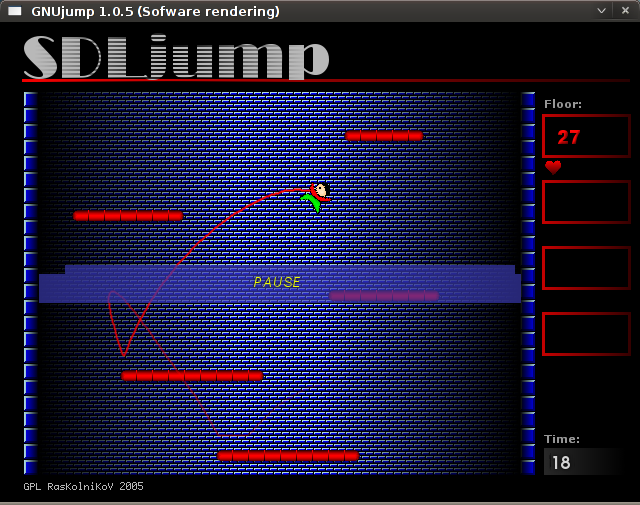
\includegraphics[width=5cm]{figs/gnujump.png}}
\end{frame}

\section{Practical session 3: packaging a Java library}
\begin{frame}{Practical session 3: packaging a Java library}
\begin{enumerate}
	\item Take a quick look at some documentation about Java packaging:\\
		\begin{itemize}
		\item \url{http://wiki.debian.org/Java}
      \hbr
		\item \url{http://wiki.debian.org/Java/Packaging}
      \hbr
		\item \url{http://www.debian.org/doc/packaging-manuals/java-policy/}
      \hbr
		\item \url{http://pkg-java.alioth.debian.org/docs/tutorial.html}
      \hbr
		\item Paper and slides from a Debconf10 talk about javahelper:\\
			{\footnotesize
			\url{http://pkg-java.alioth.debian.org/docs/debconf10-javahelper-paper.pdf}\\
			\url{http://pkg-java.alioth.debian.org/docs/debconf10-javahelper-slides.pdf}}
		\end{itemize}
		\br
	\item Download IRClib from \url{http://moepii.sourceforge.net/}
		\br
	\item Package it
\end{enumerate}
\end{frame}

\section{Practical session 4: packaging a Ruby gem}
\begin{frame}{Practical session 4: packaging a Ruby gem}
\begin{enumerate}
	\item Take a quick look at some documentation about Ruby packaging:\\
		\begin{itemize}
		\item \url{http://wiki.debian.org/Ruby}
      \hbr
		\item \url{http://wiki.debian.org/Teams/Ruby}
      \hbr
		\item \url{http://wiki.debian.org/Teams/Ruby/Packaging}
      \hbr
		\item \texttt{gem2deb(1)}, \texttt{dh\_ruby(1)} (in the \texttt{gem2deb} package)
		\end{itemize}
		\hbr
	\item Create a basic Debian source package from the \texttt{net-ssh} gem:\\
		\texttt{gem2deb net-ssh}
	\hbr
	\item Improve it so that it becomes a proper Debian package
\end{enumerate}
\end{frame}

\section{Answers to practical sessions}

\begin{frame}
	\begin{center}
		\LARGE Answers to\\[0.5em]  practical sessions
	\end{center}
\end{frame}


\subsection{Practical session 1: modifying the grep package}

\begin{frame}{Practical session 1: modifying the grep package}
\begin{enumerate}
  \item Go to \url{http://ftp.debian.org/debian/pool/main/g/grep/} and
    download version 2.6.3-3 of the package (if you use Ubuntu 11.10 or
    later, or Debian testing or unstable, use version 2.9-1 or 2.9-2 instead)

	\item Look at the files in \texttt{debian/}.
		\begin{itemize}
			\item 		How many binary packages are generated by this source package?
			\item 		Which packaging helper does this package use?
		\end{itemize}
    \hbr
	\item Build the package
    \hbr
	\item We are now going to modify the package. Add a changelog entry and increase the version number.
    \hbr
	\item Now disable perl-regexp support (it is a \texttt{./configure} option)
    \hbr
	\item Rebuild the package
    \hbr
	\item Compare the original and the new package with debdiff
    \hbr
	\item Install the newly built package
    \hbr
	\item Cry if you messed up ;)
\end{enumerate}
\end{frame}

\begin{frame}{Fetching the source}
\begin{enumerate}
	\item Go to \url{http://ftp.debian.org/debian/pool/main/g/grep/} and
		download version 2.6.3-3 of the package
\end{enumerate}
\begin{itemize}
	\item Use dget to download the \texttt{.dsc} file:\\
		{\small \texttt{dget http://cdn.debian.net/debian/pool/main/g/grep/grep\_2.6.3-3.dsc}}
		\hbr
	\item According to \url{http://packages.qa.debian.org/grep}, \texttt{grep} version 2.6.3-3 is currently in \textsl{stable} (\textsl{squeeze}). If you have \texttt{deb-src} lines for \textsl{squeeze} in your \texttt{/etc/apt/sources.list}, you can use:\\
		\texttt{apt-get source grep=2.6.3-3}\\
		or \texttt{apt-get source grep/stable}\\
		or, if you feel lucky: \texttt{apt-get source grep}
	\hbr
	\item The \texttt{grep} source package is composed of three files:
		\begin{itemize}
			\item \texttt{grep\_2.6.3-3.dsc}
			\item \texttt{grep\_2.6.3-3.debian.tar.bz2}
			\item \texttt{grep\_2.6.3.orig.tar.bz2}
		\end{itemize}
		This is typical of the "3.0 (quilt)" format.
	\hbr
\item If needed, uncompress the source with\\
	\texttt{dpkg-source -x grep\_2.6.3-3.dsc}
\end{itemize}
\end{frame}

\begin{frame}{Looking around and building the package}
	\begin{enumerate}
			\setcounter{enumi}{1}
	\item Look at the files in \texttt{debian/}.
		\begin{itemize}
			\item 		How many binary packages are generated by this source package?
			\item 		Which packaging helper does this package use?
		\end{itemize}
	\end{enumerate}
	\hbr
	\begin{itemize}
		\item According to \texttt{debian/control}, this package only generates one binary package, named \texttt{grep}.
			\hbr
		\item According to \texttt{debian/rules}, this package is typical of \textsl{classic} debhelper packaging, without using \textsl{CDBS} or \textsl{dh}. One can see the various calls to \texttt{dh\_*} commands in \texttt{debian/rules}.
	\end{itemize}
	\hbr
	\begin{enumerate}
			\setcounter{enumi}{2}

		\item Build the package
	\end{enumerate}
	\hbr
	\begin{itemize}
		\item Use \texttt{apt-get build-dep grep} to fetch the build-dependencies
		\item Then \texttt{debuild} or \texttt{dpkg-buildpackage -us -uc} (Takes about 1 min)
	\end{itemize}
\end{frame}

\begin{frame}{Editing the changelog}
	\begin{enumerate}
			\setcounter{enumi}{3}

	\item We are now going to modify the package. Add a changelog entry and increase the version number.
	\end{enumerate}
	\hbr
	\begin{itemize}
		\item \texttt{debian/changelog} is a text file. You could edit it and add a new entry manually.
	\hbr
		\item Or you can use \texttt{dch -i}, which will add an entry and open the editor
	\hbr
		\item The name and email can be defined using the \texttt{DEBFULLNAME} and \texttt{DEBEMAIL} environment variables
	\hbr
		\item After that, rebuild the package: a new version of the package is built
	\hbr
		\item Package versioning is detailed in section 5.6.12 of the Debian policy\\
			\url{http://www.debian.org/doc/debian-policy/ch-controlfields}
	\end{itemize}
\end{frame}

\begin{frame}{Disabling Perl regexp support and rebuilding}
	\begin{enumerate}
			\setcounter{enumi}{4}

	\item Now disable perl-regexp support (it is a \texttt{./configure} option)
	\item Rebuild the package
	\end{enumerate}
	\hbr
	\begin{itemize}
	  \item Check with \texttt{./configure -{}-help}: the option to disable
	    Perl regexp is \texttt{-{}-disable-perl-regexp}
	\hbr
		\item Edit \texttt{debian/rules} and find the \texttt{./configure} line
	\hbr
		\item Add \texttt{-{}-disable-perl-regexp}
	\hbr
		\item Rebuild with \texttt{debuild} or \texttt{dpkg-buildpackage -us -uc}
	\end{itemize}
\end{frame}

\begin{frame}{Comparing and testing the packages}
	\begin{enumerate}
			\setcounter{enumi}{6}

	\item Compare the original and the new package with debdiff
	\item Install the newly built package
	\end{enumerate}
	\hbr
	\begin{itemize}
		\item Compare the binary packages: \texttt{debdiff ../*changes}
	\hbr
		\item Compare the source packages: \texttt{debdiff ../*dsc}
	\hbr
		\item Install the newly built package: \texttt{debi}\\
			Or \texttt{dpkg -i ../grep\_<TAB>}
	\hbr
		\item \texttt{grep -P foo} no longer works!
	\end{itemize}
\br
\begin{enumerate}
		\setcounter{enumi}{8}
	\item Cry if you messed up ;)
\end{enumerate}
\hbr
Or not: reinstall the previous version of the package:
\begin{itemize}
	\item \texttt{apt-get install -{}-reinstall grep=2.6.3-3} \textit{(= previous version)}
\end{itemize}
\end{frame}

\subsection{Practical session 2: packaging GNUjump}
\begin{frame}{Practical session 2: packaging GNUjump}
\begin{enumerate}
	\item Download GNUjump 1.0.8 from
		\url{http://ftp.gnu.org/gnu/gnujump/gnujump-1.0.8.tar.gz}
		\br
	\item Create a Debian package for it
		\begin{itemize}
			\item Install build-dependencies so that you can build the package
			\item Get a basic working package
			\item Finish filling \texttt{debian/control} and other files
		\end{itemize}
		\br
	\item Enjoy
\end{enumerate}
\centerline{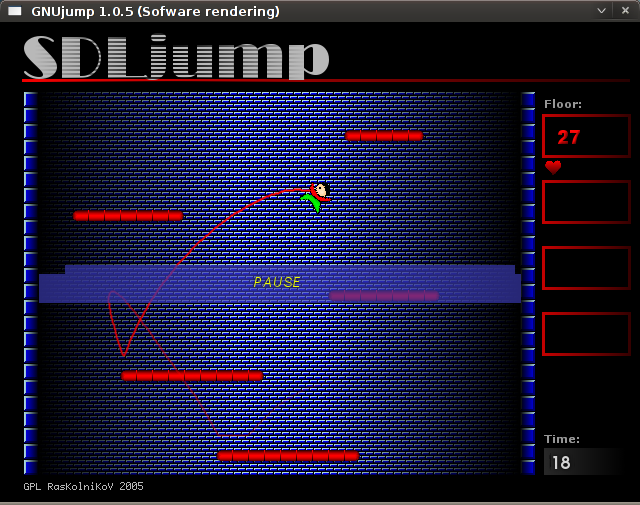
\includegraphics[width=5cm]{figs/gnujump.png}}
\end{frame}

\begin{frame}[fragile=singleslide]{Step by step\ldots}
\begin{itemize}
	\item \texttt{wget http://ftp.gnu.org/gnu/gnujump/gnujump-1.0.8.tar.gz}
		\hbr
	\item \texttt{mv gnujump-1.0.8.tar.gz gnujump\_1.0.8.orig.tar.gz}
		\hbr
	\item \texttt{tar xf gnujump\_1.0.8.orig.tar.gz}
		\hbr
	\item \texttt{cd gnujump-1.0.8/}
		\hbr
	\item \texttt{dh\_make}
	\begin{itemize}
		\item \small Type of package: single binary (for now)
	\end{itemize}
\end{itemize}
\begin{lstlisting}[basicstyle=\ttfamily\small]
gnujump-1.0.8$ ls debian/
changelog           gnujump.default.ex   preinst.ex
compat              gnujump.doc-base.EX  prerm.ex
control             init.d.ex            README.Debian
copyright           manpage.1.ex         README.source
docs                manpage.sgml.ex      rules
emacsen-install.ex  manpage.xml.ex       source
emacsen-remove.ex   menu.ex              watch.ex
emacsen-startup.ex  postinst.ex
gnujump.cron.d.ex   postrm.ex
\end{lstlisting}
\end{frame}

\begin{frame}[fragile=singleslide]{Step by step\ldots (2)}
\begin{itemize}
	\item Look at \texttt{debian/changelog}, \texttt{debian/rules}, \texttt{debian/control}\\
		(auto-filled by \textbf{dh\_make})
		\hbr
	\item In \texttt{debian/control}:\\
		\texttt{Build-Depends: debhelper (>= 7.0.50~), autotools-dev}\\
		Lists the \textsl{build-dependencies} = packages needed to build the package
		\hbr
	\item Try to build the package as-is (thanks to \textbf{dh} magic)
		\begin{itemize}
			\item And add build-dependencies, until it builds
			\item Hint: use \texttt{apt-cache search} and \texttt{apt-file} to find the packages
			\item Example:
\begin{lstlisting}[basicstyle=\ttfamily\footnotesize]
checking for sdl-config... no
checking for SDL - version >= 1.2.0... no
[...]
configure: error: *** SDL version 1.2.0 not found!
\end{lstlisting}
$\rightarrow$ Add \textbf{libsdl1.2-dev} to Build-Depends and install it.
		\hbr
	\item Better: use \textbf{pbuilder} to build in a clean environment
		\end{itemize}
\end{itemize}
\end{frame}

\begin{frame}{Step by step\ldots (3)}
\begin{itemize}
	\item After installing \texttt{libsdl1.2-dev, libsdl-image1.2-dev, libsdl-mixer1.2-dev}, the package builds fine.
		\hbr
	\item Use \texttt{debc} to list the content of the generated package.
		\hbr
	\item Use \texttt{debi} to install it and test it.
		\hbr
	\item Test the package with \texttt{lintian}
		\begin{itemize}
			\item While not a strict requirement, it is recommended that packages uploaded to Debian are \textsl{lintian-clean}
		\hbr
			\item More problems can be listed using \texttt{lintian -EviIL +pedantic}
		\hbr
			\item Some hints:
				\begin{itemize}
					\item Remove the files that you don't need in \texttt{debian/}
		\hbr
					\item Fill in \texttt{debian/control}
						\hbr
					\item Install the executable to \texttt{/usr/games} by overriding \texttt{dh\_auto\_configure}
		\hbr
					\item Use \textsl{hardening} compiler flags to increase security.\\ See \url{http://wiki.debian.org/Hardening}
				\end{itemize}
		\end{itemize}
\end{itemize}
\end{frame}

\begin{frame}{Step by step\ldots (4)}
		\begin{itemize}
	\item Compare your package with the one already packaged in Debian:
		\begin{itemize}
			\item It splits the data files to a second package, that is the same across all architectures ($\rightarrow$ saves space in the Debian archive)
				\hbr
			\item It installs a .desktop file (for the GNOME/KDE menus) and also integrates into the Debian menu
				\hbr
			\item It fixes a few minor problems using patches
		\end{itemize}
\end{itemize}
\end{frame}

\subsection{Practical session 3: packaging a Java library}
\begin{frame}{Practical session 3: packaging a Java library}
\begin{enumerate}
	\item Take a quick look at some documentation about Java packaging:\\
		\begin{itemize}
		\item \url{http://wiki.debian.org/Java}
      \hbr
		\item \url{http://wiki.debian.org/Java/Packaging}
      \hbr
		\item \url{http://www.debian.org/doc/packaging-manuals/java-policy/}
      \hbr
		\item \url{http://pkg-java.alioth.debian.org/docs/tutorial.html}
      \hbr
		\item Paper and slides from a Debconf10 talk about javahelper:\\
			{\footnotesize
			\url{http://pkg-java.alioth.debian.org/docs/debconf10-javahelper-paper.pdf}\\
			\url{http://pkg-java.alioth.debian.org/docs/debconf10-javahelper-slides.pdf}}
		\end{itemize}
		\br
	\item Download IRClib from \url{http://moepii.sourceforge.net/}
		\br
	\item Package it
\end{enumerate}
\end{frame}

\begin{frame}{Step by step\ldots}
\begin{itemize}
	\item \texttt{apt-get install javahelper}
		\hbr
	\item Create a basic source package: \texttt{jh\_makepkg}
		\begin{itemize}
			\item Library
			\item None
			\item Default Free compiler/runtime
		\end{itemize}
		\hbr
	\item Look at and fix \texttt{debian/*}
		\hbr
	\item \texttt{dpkg-buildpackage -us -uc} or \texttt{debuild}
		\hbr
	\item \texttt{lintian}, \texttt{debc}, etc.
		\hbr
	\item Compare your result with the \texttt{libirclib-java} source package
\end{itemize}
\end{frame}

\subsection{Practical session 4: packaging a Ruby gem}
\begin{frame}{Practical session 4: packaging a Ruby gem}
\begin{enumerate}
	\item Take a quick look at some documentation about Ruby packaging:\\
		\begin{itemize}
		\item \url{http://wiki.debian.org/Ruby}
      \hbr
		\item \url{http://wiki.debian.org/Teams/Ruby}
      \hbr
		\item \url{http://wiki.debian.org/Teams/Ruby/Packaging}
      \hbr
		\item \texttt{gem2deb(1)}, \texttt{dh\_ruby(1)} (in the \texttt{gem2deb} package)
		\end{itemize}
		\hbr
	\item Create a basic Debian source package from the \texttt{net-ssh} gem:\\
		\texttt{gem2deb net-ssh}
	\hbr
	\item Improve it so that it becomes a proper Debian package
\end{enumerate}
\end{frame}

\begin{frame}{Step by step\ldots}
\texttt{gem2deb net-ssh}:
\begin{itemize}
\item Downloads the gem from rubygems.org
\item Creates a suitable .orig.tar.gz archive, and untar it
\item Initializes a Debian source package based on the gem's metadata
	\begin{itemize}
		\item Named \texttt{ruby-\textsl{gemname}}
	\end{itemize}
\item Tries to build the Debian binary package (this might fail)
\end{itemize}
\br
\texttt{dh\_ruby} (included in \textsl{gem2deb}) does the Ruby-specific tasks:
\begin{itemize}
	\item Build C extensions for each Ruby version
	\item Copy files to their destination directory
	\item Update shebangs in executable scripts
	\item Run tests defined in \texttt{debian/ruby-tests.rb} or \texttt{debian/ruby-test-files.yaml}, as well as various other checks
\end{itemize}
\end{frame}

\begin{frame}[fragile=singleslide]{Step by step\ldots (2)}
Improve the generated package:
\begin{itemize}
	\item Run \texttt{debclean} to clean the source tree. Look at \texttt{debian/}.
		\hbr
	\item \texttt{changelog} and \texttt{compat} should be correct
		\hbr
	\item Edit \texttt{debian/control}: uncomment \texttt{Homepage}, improve \texttt{Description}
		\hbr
	\item Write a proper \texttt{copyright} file based on the upstream files
		\hbr
	\item \texttt{ruby-net-ssh.docs}: install \texttt{README.rdoc}
		\hbr
%Translators:
%This context is very sensitive to line length. If you
%hit errors building the package around this line in your translated version
%see, e.g. in the Spanish or German version for versions with explicit line
%breaks for the translation
	\item \texttt{ruby-tests.rb}: run the tests. In that case, it is enough to do:\\
		\verb+$: << 'test' << 'lib' << '.'+\\
		\verb+require 'test/test_all.rb'+
\end{itemize}
\end{frame}

\begin{frame}[fragile=singleslide]{Step by step\ldots (3)}
Build the package.
It fails to build. There are two problems:
\begin{itemize}
	\item You need to disable the \texttt{gem} call in the test suite.\\
	In \texttt{test/common.rb}, remove the \verb+gem "test-unit"+ line:
		\begin{itemize}
			\item \texttt{edit-patch disable-gem.patch}
			\item Edit \texttt{test/common.rb}, remove the \texttt{gem} line. Exit the sub-shell
			\item Describe the changes in \texttt{debian/changelog}
			\item Document the patch in \texttt{debian/patches/disable-gem.patch}
		\end{itemize}
		\hbr

	\item The package lacks a build-dependency on \texttt{ruby-mocha},
		which is used by the test suite (you might need to build your
		package in a clean environment, using \texttt{pbuilder}, to
		reproduce that problem)

		\begin{itemize}
			\item Add \texttt{ruby-mocha} to the package's \texttt{Build-Depends}

			\item \textsl{gem2deb} copies the dependencies
				documented in the \textsl{gem} as comments in
				\texttt{debian/control}, but \textsl{mocha} is
				not listed as a development dependency by the
				gem (that's a bug in the gem)
		\end{itemize}
\end{itemize}
\hbr
Compare your package with the \texttt{ruby-net-ssh} package in the Debian archive
\end{frame}

\end{document}
